\section{Triangulations}
Triangulations are a key tool in the process of curve reconstruction. Specifically, a type of triangulation called a Delaunay triangulation is used to construct the crust of a given set of points. Before diving into Delaunay triangulations and some interesting results that follow, we first explore an easier problem, the triangulation of a polygon, and build up to Delaunay triangulations from there.

\subsection{Triangulations of Polygons}

To begin, we must first define a triangulation of a polygon. \begin{definition}
	\textbf{Triangulation of a Polygon in two dimensions} A decomposition of a polygon into triangles by a maximal set of non-intersecting diagonals.
\end{definition}

In simpler terms, a triangulation breaks a polygon into triangular pieces by drawing segments between its vertices so that no two segments intersect. The term 'maximal set' is used in the definition to ensure that there is no vertex of the polygon on the edge of any triangle.

As an example, let's look at an easy case: a convex octagon. It is easy to pick out a way to triangulate this shape: just start at one vertex and draw lines to every other vertex as shown in \figref{fig_example_triangulations}. It is easy to see how this technique can extend to any convex n-gon to create a triangulation with n-2 triangles. Something of note is that there can be more than one way to triangulate a polygon, with another example shown in \figref{fig_example_triangulations}. Is it possible that some triangulations are better than others? The fact that there is a section dedicated to a specific type, the Delaunay triangulation, should be a clue here, and the reason why is explored in that section.

\begin{figure}
\[
    \begin{tikzpicture}
      % regular octagon as a node; change minimum size to scale
      \node[
        draw,
        thick,
        regular polygon,
        regular polygon sides=8,
        minimum size=4cm,    % controls overall size
        rotate=22.5          % optional: rotate so a side is horizontal
      ] (oct1) at (-3,0) {};
    
        % regular octagon as a node; change minimum size to scale
      \node[
        draw,
        thick,
        regular polygon,
        regular polygon sides=8,
        minimum size=4cm,    % controls overall size
        rotate=22.5          % optional: rotate so a side is horizontal
      ] (oct2) at (4,0) {};
      
      \foreach \i in {1,...,8}{
        \fill (oct1.corner \i) circle (1.5pt);
        \fill (oct2.corner \i) circle (1.5pt);
      }
      \foreach \i in {1,5,6,7,8}{
        \draw[black, very thick] (oct1.corner 3) -- (oct1.corner \i);
      }
      \draw[black, very thick] (oct2.corner 4) -- (oct2.corner 2);
      \draw[black, very thick] (oct2.corner 4) -- (oct2.corner 1);
      \draw[black, very thick] (oct2.corner 1) -- (oct2.corner 5);
      \draw[black, very thick] (oct2.corner 1) -- (oct2.corner 6);
      \draw[black, very thick] (oct2.corner 8) -- (oct2.corner 6);

    
    \end{tikzpicture}
\]
\caption{Two example triangulations of a regular octagon.} \label{fig_example_triangulations}
\end{figure}

A more interesting problem arises when you try to triangulate a shape that is nonconvex. Is this even possible for \textit{any} polygon? If it is, is there an algorithmic way that works to triangulate any polygon? Will there always be the same number of triangles? The following theorems dive deeper into these questions.

\begin{theorem}All polygons can be triangulated\end{theorem}

\begin{proof}  %This proof comes from computational geometry by springer
	This is an inductive proof with the base case being a polygon with 3 vertices. This base case is trivial because a triangle need not be broken down into more triangular pieces. Now, the assumption that any polygon with $m$ or fewer vertices can be triangulated and our goal is to show that that a polygon with $n$ vertices with $n = m+1 > 3$ can be triangulated.

	I will begin by showing that a diagonal exists in the polygon, $P$, formed by $n$ vertices. Take some vertex $v$ from $P$ and label the vertices neighboring it $u$ and $w$. If $u$ and $w$ are connected and do not intersect with any edges of $P$, then a diagonal exists. Otherwise, there exists one ore more vertices of $P$ that are inside triangle $uvw$. Now, imagine a line parallel to segment $uw$ that goes through $v$. Let this line sweep toward segment $uw$ until it encounters a vertex of $P$ inside triangle $uvw$ and call this vertex $v'$. The segment $vv'$ must be a diagonal because there are no edges of $P$ between $v$ and $v'$ by the definition of $v'$. So, a diagonal must exist in $P$.

	The existence of this diagonal means that $P$ can be broken into two polygons that share the diagonal as a common edge, with a total of $n+2$ vertices. There are $n+2$ because the $n$ outer edges of the polygon remain part of either new polygon, and the diagonal contributes one edge to each of the newly created polygon, adding two edges. Since each new polygon must have at least 3 vertices, the other must have at most $n-1 = m$ vertices. By the inductive hypothesis, each of these new polygons may be triangulated.

	
\newcommand{\nextindex}[3]{%
  % #1 = current index
  % #2 = maximum index
  % #3 = name of variable to store result
  \pgfmathtruncatemacro{\temp}{#1+1}%
  \ifnum\temp>#2
    \pgfmathtruncatemacro{#3}{1}%
  \else
    \pgfmathtruncatemacro{#3}{\temp}%
  \fi
}

\begin{figure}
\[
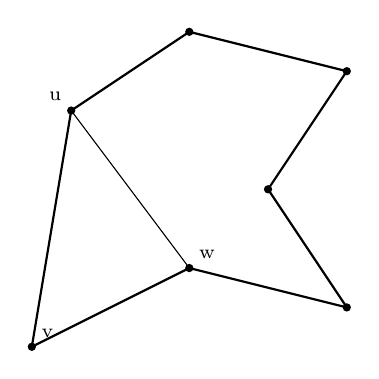
\begin{tikzpicture}[scale=1]
  \coordinate (P1) at (0,0);
  \coordinate (P2) at (2,1);
  \coordinate (P3) at (4,0.5);
  \coordinate (P4) at (3,2);
  \coordinate (P5) at (4,3.5);
  \coordinate (P6) at (2,4);
  \coordinate (P7) at (0.5,3);

  \foreach \i in {1,...,7} {
    \nextindex{\i}{7}{\next}
    \draw[thick] (P\i) -- (P\next);
    \fill (P\i) circle (1.5pt);
  }
  \node[font=\scriptsize, above right] at (P1) {v};
  \node[font=\scriptsize, above right] at (P2) {w};
  \node[font=\scriptsize, above left] at (P7) {u};

  \draw[thin]
    (P2) -- (P7);
  
\end{tikzpicture}
\hspace{3cm}
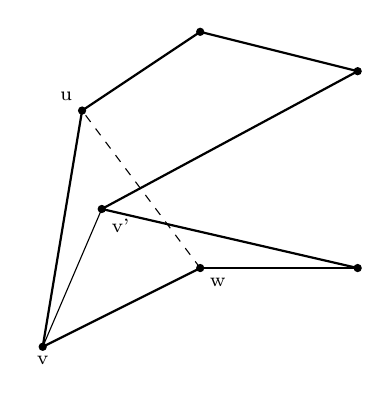
\begin{tikzpicture}[scale=1]
  % --- Define 7 vertices of a nonconvex heptagon ---
  % (Change numbers as you like)
  \coordinate (P1) at (0,0);
  \coordinate (P2) at (2,1);
  \coordinate (P3) at (4,1);
  \coordinate (P4) at (.75,1.75);
  \coordinate (P5) at (4,3.5);
  \coordinate (P6) at (2,4);
  \coordinate (P7) at (0.5,3);

  \foreach \i in {1,...,7} {
    \nextindex{\i}{7}{\next}
    \draw[thick] (P\i) -- (P\next);
    \fill (P\i) circle (1.5pt);
  }
  \node[font=\scriptsize, below] at (P1) {v};
  \node[font=\scriptsize, below right] at (P2) {w};
  \node[font=\scriptsize, above left] at (P7) {u};
  \node[font=\scriptsize, below right] at (P4) {v'};
  
  \draw[dashed]
    (P2) -- (P7);
  \draw[thin]
    (P1) -- (P4);
  
\end{tikzpicture}
\]
\caption{The two cases when trying to draw a diagonal between two points around a starting point.} \label{fig_diagonal_creation}
\end{figure}
\end{proof}

In the process of proving that it is always possible to triangulate any polygon, we have also generated a simple algorithm to triangulate any polygon. If we begin the same way as the proof, drawing a diagonal between some pair of vertices, two smaller shapes are created. Each of these shapes can undergo the same process and create two more shapes. This can be repeated recursively until all the shapes created by the splits are just triangles, so all the diagonals drawn must constitute a triangulation.
\subsection{Triangulations of a Set of Points}

In the previous section, I showed that any polygon can be triangulated. The method to do this started by drawing a single new edge to form a triangle using two preexisting edges. But what if there are no edges at all, and you just have a set of points? You could construct any number of polygons for a given set of points. To make this algorithmic, we must choose a specific one of these polygons to start to triangulate. To do this, we return to the familiar convex hull.

\begin{definition}
	\textbf{Triangulation of a set of Points} FILL OUT THIS DEFINITION
\end{definition}

After computing the convex hull, our situation appears almost like it did in the previous section, but there are still points inside that are not accounted for. To continue down this path, we sincerely hope that the following theorem is true:

\begin{theorem}
	Any set of points $S$ has a triangulation, $T$, such that \textit{Hull(S)}$ \subset T$. --- notation might not be quite right here, we want the edges of the hull to be a part of the edges of T
\end{theorem}

\begin{proof}

	We follow a similar method to the previous proof, using induction. Again, the base case is a set of 3 points, with the obvious triangulation of a triangle, which is also the convex hull of the points. Our hypothesis is that, assuming that a set of points $S$ of size $n$ has triangulation $T$ with \textit{Hull(S)}$ \subset T$, some $S' \supset S$ of size $n+1$ has triangulation $T'$ with \textit{Hull(S')}$ \subset T'$.

	There are two cases for the new vertex $v$ that belongs to $S'$ but not $S$. Either $v$ is inside \textit{Hull(S)}, or it is outside of it. We will examine each case independently:

	Explain that a point outside will have a new hull with two "new edges", and if these two edges are added to the previous triangulation, we still have a triangulation.

	Explain how a point inside the hull is in a triangle, and hence this triangle can just have each vertex connect to the point inside and maintain a triangulation

	...

\end{proof}

\subsection{Delaunay Triangulations}
Now that we know that we can generate some triangulation for any set of points, we can begin to look at a certain type of triangulation, the Delaunay Triangulation. The Delaunay Triangulation of a set of points has interesting properties and is the primary tool in generating the crust of a given set of points. But before we explore those properties, let us first define it.

\begin{definition}
	A \textbf{Delaunay Triangulation} is the triangulation of a set of points $S$ such that the circumcircle of each triangle only contains the vertices of that triangle, and no other points in $S$
\end{definition}
\begin{figure}
\centering

\begin{subfigure}{0.45\textwidth}
\centering
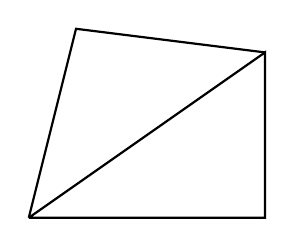
\begin{tikzpicture}[scale=3]
    
    \coordinate (A) at (0,0);
    \coordinate (B) at (1,0);
    \coordinate (C) at (0.2,0.8);
    \coordinate (D) at (1,0.7);
    
    \draw[thick] (A)--(B)--(D)--(A);
    \draw[thick] (A)--(C)--(D);
\end{tikzpicture}
\caption{Non-Delaunay Triangulation}
\end{subfigure}

\hfill

\begin{subfigure}{0.45\textwidth}
\centering
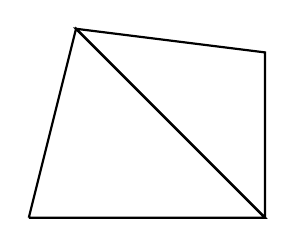
\begin{tikzpicture}[scale=3]    
    % Same points
    \coordinate (A) at (0,0);
    \coordinate (B) at (1,0);
    \coordinate (C) at (0.2,0.8);
    \coordinate (D) at (1,0.7);
    
    % Triangulation (Delaunay: diagonal BC)
    \draw[thick] (A)--(B)--(C)--(A);
    \draw[thick] (B)--(C)--(D)--(B);
\end{tikzpicture}
\caption{Delaunay Triangulation}
\end{subfigure}

\end{figure}


Something you may have noticed in the definition of a Delaunay triangulation is that I claimed that it is \textit{the} triangulation that fits the criteria, not just some triangulation that does. This uniqueness is an important property of Delaunay Triangulations, but it is not at all apparent. Let us show why this is true:

SHOW THAT THE EXISTENCE IS ALSO GUARANTEED

\begin{theorem}
	There is only one Delaunay Triangulation for given set of points $S$.
\end{theorem}
\begin{proof}

\end{proof}

It is of note that if there are four points that are concentric, then there cannot be a triangulation that fits the Delaunay criteria. So, the four points have, in some sense, two valid Delaunay triangulations. We call these triangulations degenerate.

Another interesting property of Delaunay triangulations is that they guarantee that the smallest internal angle of any triangle in the shape is the highest out of all possible triangulations.

\begin{theorem}
	The Delaunay Triangulation has the highest minimum internal angle out of all possible triangulations
\end{theorem}
\begin{proof}

\end{proof}
Effectively, Delaunay triangulations reduce "sliver triangles" which are very long, thin triangles.

talk about angle sequences and transition that into "flipping"

show how you can get from one triangulation to the Delaunay triangulation using progressive steps

dive into talking about the 'flip graph'

show the connection to voronoi diagrams
